\subsection{Quantum computing overview}\label{subsec:17-quantum-computing-overview}

\subsubsection{Qubit notation exploiting binary representation}

For a general state, we already saw that we can write: 
\begin{equation*}
\ket{\psi} = a \, \ket{0}+b\, \ket{1}; \hspace{2ex} |a|^2+|b|^2 = 1
\end{equation*}

We can define the \textbf{quantum-register} as a collection of qubits; for example, the following 3-qubit register is:
\begin{equation}\label{eqn:16-5-in-binary-representation}
\ket{1}\otimes\ket{0}\otimes\ket{1} \equiv 
\ket{101} \coloneqq \ket{5}
\end{equation}

It represents $5$ in binary representation: $(5)_{10} = (101)_2$\footnote{The pedice $_{10}$ stands for base $10$ while $_{2}$ stands for base $2$.}.

If the first qubit is itself in a superposition:
\begin{equation*}
\frac{1}{\sqrt{2}}\,\bigl(\ket{0}+\ket{1}\bigr)
\end{equation*}

The register would be:
\begin{equation*}
\frac{1}{\sqrt{2}}\,
\bigl(\ket{0}+\ket{1}\bigr) \, \ket{0}\ket{1} = 
\frac{1}{\sqrt{2}}\, 
\bigl(\ket{001}+\ket{101}\bigr) = 
\frac{1}{\sqrt{2}}\, 
\bigl(\ket{1}+\ket{5}\bigr)
\end{equation*}

We obtain a simultaneous representation of two numbers. 

\question{What happens when all three qubits are in a superposition state?}{%
\begin{gather*}
\frac{1}{\sqrt{2}}\,
\bigl(\ket{0}+\ket{1}\bigr) \otimes
\frac{1}{\sqrt{2}}\,
\bigl(\ket{0}+\ket{1}\bigr) \otimes
\frac{1}{\sqrt{2}}\,
\bigl(\ket{0}+\ket{1}\bigr) =
\\
= \frac{1}{\sqrt{2^3}}\, 
\bigl(
    \ket{000}+\ket{001}+\ket{010}+\ket{011}+
    \ket{100}+\ket{101}+\ket{110}+\ket{111}
\bigr) =
\\
= \frac{1}{\sqrt{2^3}}\, 
\bigl(
    \ket{0}+\ket{1}+\ket{2}+\ket{3} +
    \ket{4}+\ket{5}+\ket{6}+\ket{7}
\bigr)
\end{gather*}

Which represents the quantum superposition of $8$ decimal numbers, this let us understand why quantum operations scale drastically computing power. The most general quantum computing register is indeed:
\begin{equation}\label{16-most-general-quantum-register}
\ket{\psi_N} = 
\bigotimes_{i=0}^{N-1} \, 
\frac{1}{\sqrt{2}} 
\bigl(
    \ket{0}_i + \ket{1}_i
\bigr) \equiv
\sum_{n=0}^{2^{N} - 1} 
\frac{1}{\sqrt{2^{N}}} \, \ket{n}
\end{equation}

where $i$ indexes the qubits in the quantum register, while $n$ is the decimal representation of the binary string (a.k.a. \emph{bitstring}) formed by the qubits. 
}

\subsubsection{Brief review of quantum computing} 

In a quantum register, information is encoded in the amplitudes of a state vector, whose description grows exponentially with the number of qubits, since \hl{an $N$-qubit system lives in a Hilbert space of dimension $2^N$}. This is the origin of the potential advantage over classical bits, whose description scales only linearly with $N$. 

\calloutinfo{%}
    The challenge is therefore to exploit this parallelism while preserving the quantum information and preventing decoherence. A quantum computer consists of a set of $N$ qubits whose state is manipulated by unitary operators, which are called \textbf{quantum gates}; a sequence of such gates forms a \textbf{quantum circuit}. 

    Through \textbf{quantum interference}, some amplitudes can be enhanced while others are canceled, and the goal is to combine these basic operations in a useful way, giving rise to \textbf{quantum algorithms}.
}

In a classical computer, a register stores bits of data and logic gates act on them; in the quantum case, the register is a state vector, and the circuit acts on qubits that may play the role of \textbf{control} and \textbf{target} qubits. More generally, \hl{a quantum computer is any device that uses quantum effects to perform a computational task}. The computation is described by a unitary transformation $U$, obtained as the product of elementary quantum logic operations, where unitary means\footnote{Un po' tardi dirlo solo all'ultimo capitolo no?}:
\begin{equation}\label{eqn:16-unitary-operator}
\hat{U}^\dagger \hat{U} = \hat{U}\hat{U}^\dagger = \mathbb{I},
\end{equation}

for example, the time-evolution operator
\begin{equation}\label{eqn:16-time-evolution-operator}
\hat{U}(t)=e^{-\frac{i}{\hbar}t\hat{H}}.
\end{equation}

Since unitary transformations are invertible, quantum computation is -- in principle -- \textbf{reversible}. A unitary operation evolves the quantum register while preserving the normalization of the state-vector, and therefore the quantum information stored in its amplitudes. 

The final step of a quantum computation is measurement, which extracts the result but is not unitary, since it projects the state onto one outcome and destroys the other components of the superposition. As a consequence, \hl{the result is probabilistic and the algorithm must often be repeated many times to obtain reliable statistics}. For this reason, quantum algorithms must be designed so that the amplitudes corresponding to incorrect answers interfere destructively, while the correct answer is amplified.

Finally, interaction with the environment leads to decoherence, which is also non-unitary and tends to destroy superposition and entanglement. This is why an important part of quantum computing research is devoted to error-correction and other protocols that protect quantum information from loss.

\subsubsection{Most remarkable single-qubit quantum logic gates}

\begin{enumerate}
    \item \textbf{Hadamard gate:} creates a superposition of the basis states
    \begin{equation}\label{eqn:16-hadamard-gate}
    \hat{H} = \frac{1}{\sqrt{2}}\, 
    \bigl[
        \ket{0}\bra{0}+\ket{0}\bra{1}+\ket{1}\bra{0}+\ket{1}\bra{1}
    \bigr] = 
    \frac{1}{\sqrt{2}}\, 
    \begin{pmatrix}
        1 & 1\\ 1 &-1
    \end{pmatrix}
    \end{equation}

    When applied to either state $\ket{0}$ or $\ket{1}$ leads to an equal superposition of both states. Being at the same time self-adjoint (a.k.a. \textbf{hermitian}) and unitary, it is its own inverse; thus can turn superposition states again into basis states:
    \begin{equation}
    \hat{H}\, 
    \frac{1}{\sqrt{2}}\, 
    \begin{pmatrix}
        1\\1 
    \end{pmatrix} =  \frac{1}{\sqrt{2}}\,\frac{1}{\sqrt{2}}\, \begin{pmatrix}
        1 & 1\\ 1 &-1
    \end{pmatrix}\, \begin{pmatrix}
        1\\1 
    \end{pmatrix} = \frac{1}{2}\, \begin{pmatrix}
        2\\0
    \end{pmatrix} = \begin{pmatrix}
        1\\0
    \end{pmatrix}.
    \end{equation}

    Considering Bloch sphere's representation, changing the amplitude of the qubit corresponds to operating some rotations on its position:
    \begin{enumerate}
        \item Rotation of $\pi$ about the $z$-axis;
        \item Rotation of $\frac{\pi}{2}$ about the $y$-axis.
    \end{enumerate}

    \item \textbf{X-gate:} also referred to as \textbf{not-gate}, since it switches $\ket{0}$ with $\ket{1}$ and vice versa:
    \begin{equation}\label{eqn:16-x-gate}
    \hat{X} = 
    \ket{1}\bra{0}+\ket{0}\bra{1} = 
    \begin{pmatrix}
        0 &1\\1&0
    \end{pmatrix}
    \end{equation}

    It corresponds to a rotation of $\pi$ about the $x$-axis.

    \item \textbf{Z-gate:} flips the sign of $\ket{1}$, leaving $\ket{0}$ unchanged
    \begin{equation}\label{eqn:16-z-gate}
    \hat{Z} = \ket{0}\bra{0}-\ket{1}\bra{1} = \begin{pmatrix}
        1 &0\\0&-1
    \end{pmatrix}
    \end{equation}

    It corresponds to a rotation of $\pi$ about the $z$-axis.

    \item \textbf{Y-gate:} change $\ket{0}\to i\, \ket{1}$ and $\ket{1} \to -i\, \ket{0}$
    \begin{equation}\label{eqn:16-y-gate}
    \hat{Y} = i\, \ket{1}\bra{0}-i\,\ket{0}\bra{1} = \begin{pmatrix}
        0 &-i\\i&0
    \end{pmatrix}
    \end{equation}

    It corresponds to a rotation of $\pi$ about the $y$-axis.
\end{enumerate}

As said, all these gates can be thought as some rotations on the Bloch sphere; without any formalism, we can say that they are generalized by the generic rotation:
\begin{equation}\label{eqn:16-generic-rotation}
    \hat{R}_{\phi} = \ket{0}\bra{0}+e^{i\phi}\, \ket{1}\bra{1}
\end{equation}

\subsubsection{Two-qubit gates overview and controlled operations}

The gates which operates on two or more qubits are called \textbf{controlled operations}. Suppose to have a 2 input q-bits one is control and the other is target, the gate has no effect on the control q-bit, but performs a unitary operation on the target q-bit conditionally on the state of the control q-bit.
\textbf{C-NOT gate:} (controlled-not)
\begin{equation}\label{eqn:16-cnot-gate}
\hat{C} = 
\ket{00}\bra{00} + \ket{01}\bra{01} +
\ket{10}\bra{11} + \ket{11}\bra{10} = 
\begin{pmatrix}
    1&0&0&0\\ 
    0&1&0&0\\
    0&0&0&1\\
    0&0&1&0
\end{pmatrix}
\end{equation}

If the control state is $\ket{0}$ the target state remains unchanged, while if the control state is $\ket{1}$ the target state flips whatever its initial state is. 
This gate can be written in a symbolic form as:
\begin{equation}\label{eqn:16-cnot-circuit}
\begin{quantikz}
\lstick{$\ket{c}$} & \ctrl{1} & \rstick{$\ket{c}$} \\
\lstick{$\ket{t}$} & \targ{}  & \rstick{$\ket{t \oplus c}$}
\end{quantikz}
\end{equation}

Where $\oplus$ is addition modulo $2$ \footnote{For a single-qubit state $\ket{t}$, $t$\in\{0,1\}; if $c=0$ nothing happens, whereas if $c=1$ the possibile outcomes are: $0\oplus 1 = 1$ and $1\oplus 1 = 0$}.


\subsection{Optical implementation of quantum gates}\label{subsec:17-optical-implementation-of-quantum-gates}

\question{How can we implement this with optical schemes?}{%
Quantum information is encoded onto modes occupied by single photons, which are manipulated using linear optical components such as B.S., phase shifters, etc...
}

\subsubsection{Hadamard gate through a half-wave plate}

Let's start with \textbf{Hadamard gate}: the simplest optical object that realizes it is a half-wave plate, an optical device that alters the polarization of light (here by \qty{45}{\degree}).

\begin{figure}[H]
    \centering
    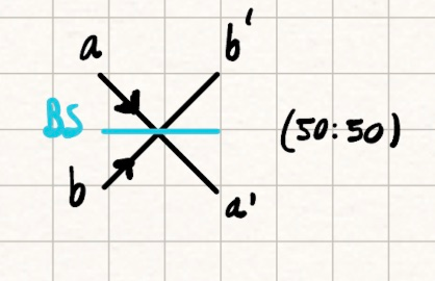
\includegraphics[width=0.4\linewidth]{images_in_pdf/17-/17-hadamard-bs.pdf}
    \caption{Hadamard gate through a half-wave plate.}
\end{figure}

\begin{equation}\label{eqn:17-dual-rail-realization-1}
\begin{cases}
    \hat{a}' = \frac{1}{\sqrt{2}}\, (\hat{a}+\hat{b})\\
    \hat{b}' = \frac{1}{\sqrt{2}}\, (\hat{a}-\hat{b})
\end{cases} \implies \hspace{2ex}
\begin{cases}
    \hat{a} = \frac{1}{\sqrt{2}}\, (\hat{a}'+\hat{b}')\\
    \hat{b} = \frac{1}{\sqrt{2}}\, (\hat{a}'-\hat{b}')
\end{cases}
\end{equation}

\subsubsection{Hadamard gate through a B.S.}

We take in consideration the \textbf{dual rail realization} (i.e. an architecture where a single bit, called \say{logical state} is represented by two physical signals) through a B.S. 

The computational states $\ket{0}$ and $\ket{1}$ are composed by the product of two states:
\begin{equation}\label{eqn:17-dual-rail-realization-2}
\ket{0} \coloneqq \ket{0}_a\ket{1}_b
\hspace{1ex} \land \hspace{1ex}
\ket{1} \coloneqq \ket{1}_a\ket{0}_b
\end{equation}

Notice that, by themselves, the vacuum and single-photon states do not compose the computational basis; it is their product that gives us the states on which we operate.

The two input modes are labeled $a$ and $b$, while the output modes are labeled $a'$ and $b'$. On our logic states, the B.S. transformation $\hat{U}_{\text{B.S.}}$ acts as:
\begin{align}
\hat{U}_{\text{B.S.}} \ket{0}_a \ket{1}_b &= 
\frac{1}{\sqrt{2}} 
\bigl( 
    \ket{0}_{a'}\ket{1}_{b'} + \ket{1}_{a'}\ket{0}_{b'} 
\bigr) = \nonumber \\
&= \frac{1}{\sqrt{2}}
\bigl(
    \ket{01} + \ket{10}
\bigr); \label{eqn:17-bs-transformation-01} \\[2ex]
%
\hat{U}_{\text{B.S.}} \ket{1}_a \ket{0}_b 
&= \frac{1}{\sqrt{2}} 
\bigl( 
    \ket{1}_{a'}\ket{0}_{b'} - \ket{0}_{a'}\ket{1}_{b'} 
\bigr) \nonumber = \\
&= \frac{1}{\sqrt{2}} 
\bigl( 
    \ket{10} - \ket{01} 
\bigr). \label{eqn:17-bs-transformation-10}
\end{align}


\subsubsection{C-NOT gate through linear optics}

Let us implement a \textbf{linear optical C-NOT} gate exploiting \textbf{polarizing beam splitters (p.B.S.)}\footnote{A polarizing beam splitter is a device that separates light into two components based on their polarization, contrary to the 50:50 variant that separates light into parts of equal intensity.}, unbalanced beam splitters (u.B.S.), half-wave plates (H.W.P.) and \emph{post-selection}.
\begin{figure}[H]
    \centering
    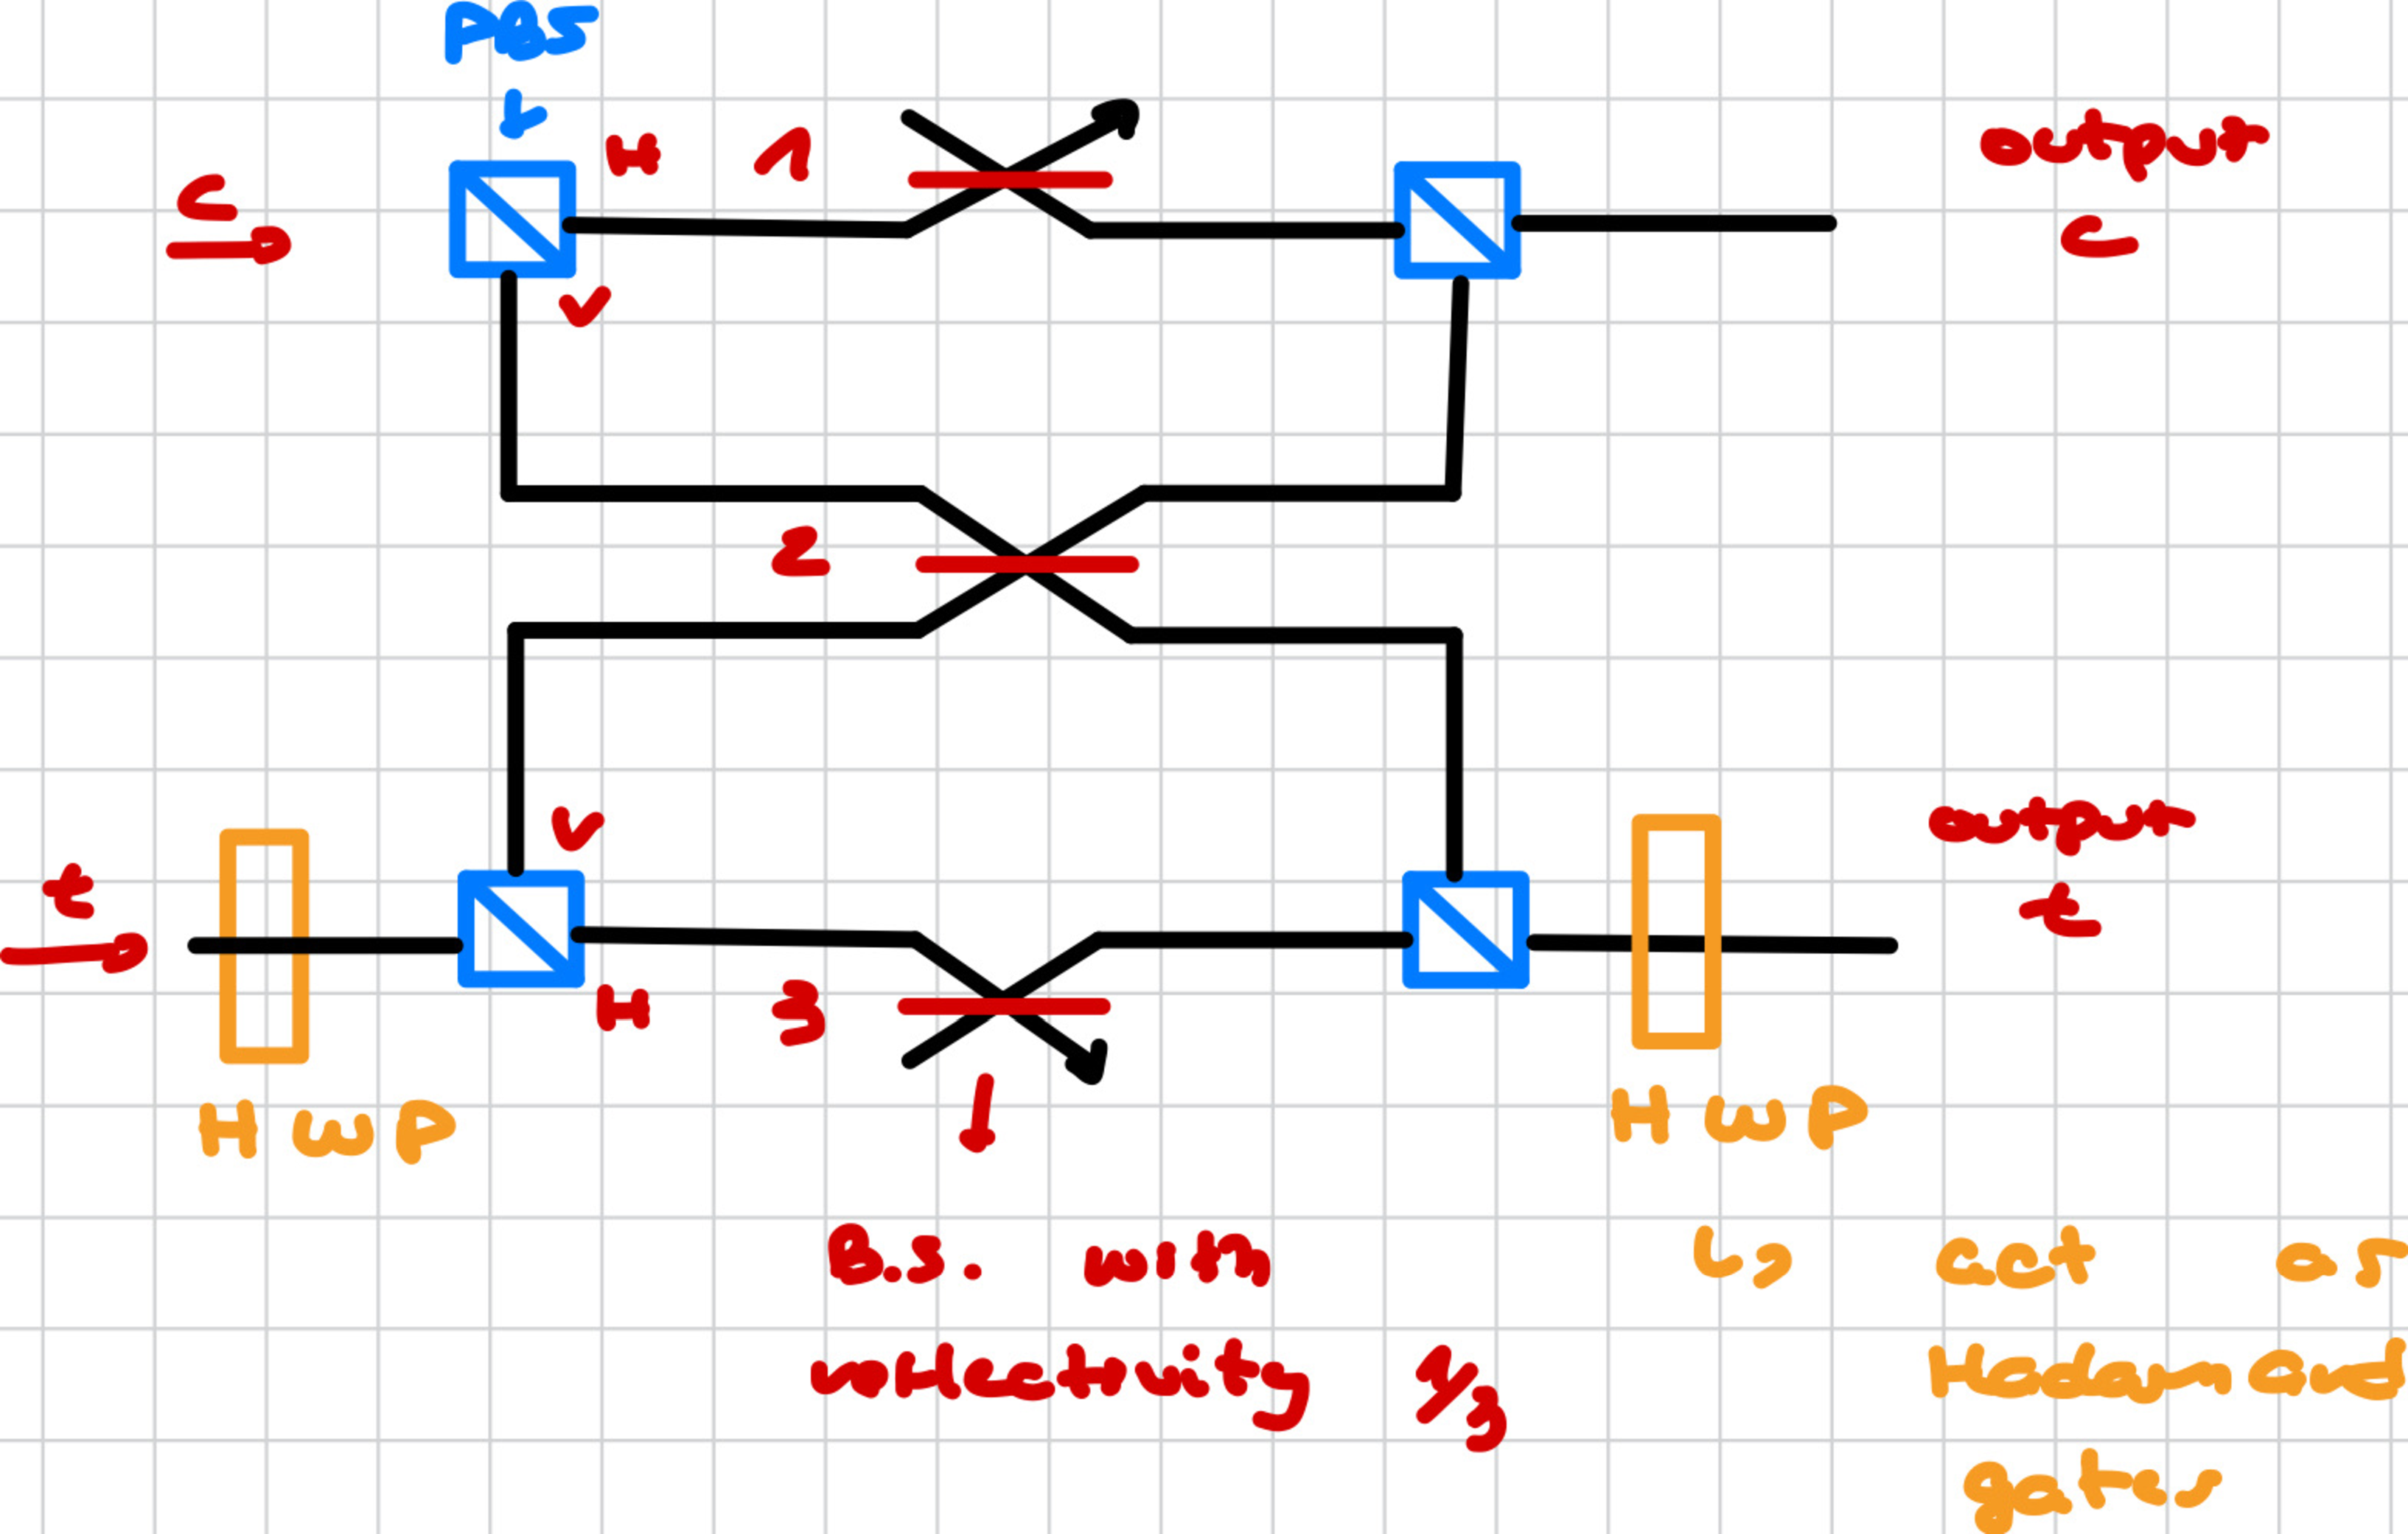
\includegraphics[width=0.6\linewidth]{images_in_pdf/17-/17-cnot-lin-opt.pdf}
    \caption{C-NOT gate through p.B.S.s, u.B.S.s, and H.W.P.s.}
\end{figure}

\begin{enumerate}
\item The \textbf{control qubit} approaches a \emph{polarizing beam splitter} \hl{which produces a horizontal (transmitted) and a vertical (reflected) component};

\item The \textbf{target qubit} approaches another \emph{polarizing beam splitter} \hl{which also produces a horizontal and a vertical component};

\item The \emph{transmitted component} of the control qubit goes to an \textbf{unbalanced B.S.} with a reflectivity of $\frac{1}{3}$ (hence $\tran=\frac{2}{3}$), then follows a path to another polarizing beam splitter, where it can give only a single output; the same happens for the transmitted part of the target qubit;

\item Both \emph{reflected components} are \textbf{mixed} in another unbalanced B.S. with the same reflectivity; the upper one goes to a polarizing beam splitter and then to the output of the control qubit, while the lower one goes to another polarizing beam splitter;

\item Now, \hl{only for the target qubit}, we add a \textbf{half-wave plate} \emph{before} the first polarizing beam splitter and \emph{another after} the second one, which act as Hadamard gates.
\end{enumerate}

To study the C-NOT behavior of this apparatus, we use \textbf{dual-rail logic}. We use a particular notation, where $c$ and $t$ will stand for the control and target qubits, respectively; a pedice $H$ or $V$ will indicate the polarization considered. In this sense, we will refer to the states $\ket{H}_c$ and $\ket{V}_c$ as:

\begin{equation}
\ket{H}_c \coloneqq \ket{0} \mapsto  
\begin{cases}
    \ket{1}_{c_H}\\
    \ket{0}_{c_V}
\end{cases} 
\end{equation}

\begin{equation}
\ket{V}_c \coloneqq \ket{1} \mapsto  
\begin{cases}
    \ket{0}_{c_H}\\
    \ket{1}_{c_V}
\end{cases} 
\end{equation}

The same will hold for the target qubit.

\calloutinfo{%
    To stress it again, a horizontal polarization corresponds to the logical state $\ket{0}$, while a vertical polarization corresponds to the logical state $\ket{1}$. The C-NOT gate should then flip the polarization of the target qubit if the control qubit's polarization is vertical, while leaving it unchanged if the control qubit's polarization is horizontal.
}

Let's unpack the behavior of this system by considering the possible input states.

\calloutwarn{%
    We only consider events where photons arrive at both the target and control outputs simultaneously (clicking the outputs simultaneously); this is called \textbf{post-selection}, i.e.: discarding all outcomes that do not satisfy the chosen criteria. This means that we do not take into account the events in which photons are transmitted by the first and third u.B.S., since it would mean the photons are exiting the system. At the same time, we also discard the events where the second u.B.S. reflects one photon while transmitting the other, since it would mean that they are exiting from the same output port.
} 

\begin{itemize}

\item[\textbf{CASE \Rnum{1}:}] \hl{both input photons are horizontally polarized}, $\ket{H}_c$ and $\ket{H}_t$. The target qubit passes through the half-wave plate, which acts as a Hadamard transformation sending it to a superposition of horizontal and vertical polarization:
\begin{equation}
\ket{H}_c\ket{H}_t 
\stackrel{\text{\tiny{H.W.P.}}}{\longrightarrow} 
\ket{H}_c \, 
\otimes
\frac{1}{\sqrt{2}}\, 
\bigl( 
    \ket{H}_t+\ket{V}_t
\bigr)
\end{equation}

When our input photons enter their first p.B.S.:

\begin{itemize}
    \item The control qubit has a definite \emph{horizontal} polarization, hence exits the p.B.S. on the top path, then gets reflected by the first u.B.S.;
    \item The target qubit was put in a superposition so, exiting the p.B.S., it can either take the middle path (making it \emph{vertical}) and get reflected by the second u.B.S. or choose the bottom path (making it \emph{horizontal}) and get reflected by the third u.B.S.
\end{itemize}

Overall, requiring two u.B.S. reflections, the amplitude of the successful components is reduced by a factor of: $\frac{1}{\sqrt{3}}\, \frac{1}{\sqrt{3}}= \frac{1}{3}$.

The output state is then:
\begin{equation}
\frac{1}{3}\, \ket{H}_c \,
\otimes
\frac{1}{\sqrt{2}} \,
\bigl( \ket{H}_t+\ket{V}_t\bigr)
\end{equation}

But now we have a second H.W.P. acting on the target qubit, making it go back from a superposition to a vertical state: $\tfrac{1}{\sqrt{2}}  \, \bigl( \ket{H}_t+\ket{V}_t\bigr)\to \ket{H}_t$.
\begin{equation}
\text{Output} = \frac{1}{3}\, \ket{H}_c\, \ket{H}_t
\end{equation}

We obtain the initial state, only with a different amplitude; this is the expected behavior of a C-NOT gate, since the control qubit is horizontal and therefore does not flip the target qubit's polarization.

\item[\textbf{CASE \Rnum{2}:}] control is horizontal and target is vertical: $\ket{H}_c\ket{V}_t$. This case is completely analogous to the previous one, and the same output is obtained.

\item[\textbf{CASE \Rnum{3}:}] control is vertical and target is horizontal: $\ket{V}_c\ket{H}_t$.

The target qubit passes through the half-wave plate, which acts as a Hadamard transformation:
\begin{equation}
\ket{V}_c\ket{H}_t 
\stackrel{\text{\tiny{H.W.P.}}}{\longrightarrow}
\ket{V}_c 
\otimes
\frac{1}{\sqrt{2}}\,
\bigl( \ket{H}_t+\ket{V}_t\bigr)
\end{equation}

\begin{itemize}
    \item The control qubit has a definite \emph{vertical} polarization, hence exits the p.B.S. on the middle path; from here, it can either be reflected or transmitted by the second u.B.S.;
    \item The target qubit was put in a superposition so, exiting the p.B.S., it can either take the middle path (making it \emph{vertical}) and then can be reflected or transmitted as well by the second u.B.S. [case \Rnum{3}\hspace{0.2ex}a.]; or choose the bottom path (making it \emph{horizontal}) where it has to be reflected by the third u.B.S. [case \Rnum{3}\hspace{0.2ex}b.];
\end{itemize}

\begin{itemize}

\item[\textbf{\Rnum{3}\hspace{0.2ex}b.}] If the target photon follows the bottom path, the coincidence is realized only if both photons are reflected by the second and third u.B.S., respectively. This simply leads to a reduction of the initial amplitude by $\frac{1}{3}$, leaving the target qubit unaltered in $\ket{H}_t$.

\item[\textbf{\Rnum{3}\hspace{0.2ex}a.}] If instead the target photon follows the middle path, we have two possible scenarios -- both in which target photon's polarization it's swapped to $\ket{V}_t$ -- involving the interface at the second u.B.S.:

\begin{enumerate}
    \item \hl{Both photons are \textbf{reflected}}: control photon is detected by the upper detector, while the target photon is detected by the lower detector; this leads to a reduction of the initial amplitude by $\frac{1}{3}$.
    
    \item \hl{Both photons are \textbf{transmitted}}: control photon is detected by the lower detector, while the target photon is detected by the upper detector; the final amplitude results multiplied by $-\frac{2}{3}$.
\end{enumerate}

\calloutwarn{%
    \textbf{Caution:} the photons are indistinguishable, there's no way to know which photon was detected by which detector! 
}

Given the indistinguishability of the photons, we must consider the total amplitude of the two sub-processes: $\frac{1}{3}-\frac{2}{3} = -\frac{1}{3}$. 

\end{itemize}

We now are left with a superposition of two target outcomes: a $\ket{H}_t$ from the \textbf{\Rnum{3}\hspace{0.2ex}b.} case and $\ket{V}_t$ from the \textbf{\Rnum{3}\hspace{0.2ex}a.} case, with a relative minus sign:

\begin{equation}\label{eqn:17-cnot-case-3-pre-hwp}
\frac{1}{\sqrt{2}}\ket{V}_c\, 
\otimes
\frac{1}{3}\,
\bigl(\ket{H}_t-\ket{V}_t\bigr)
\end{equation}

After the target qubit passes through the second half-wave plate, its superposition state is sent back to $\ket{V}_t$, and we finally obtain:
\begin{equation}
\frac{1}{\sqrt{2}}\ket{V}_c\, 
\otimes
\frac{1}{3}\,
\bigl(\ket{H}_t-\ket{V}_t\bigr)
\stackrel{\text{\tiny{H.W.P.}}}{\longrightarrow}
\frac{1}{3}
\ket{V}_c \ket{V}_t
\end{equation}

\calloutinfo{%
    The minus sign in the transmission amplitude appears because of a really good reason.
}


Overall, the probability of success (i.e. the fraction of photons that successfully implement the C-NOT operation) is:
\begin{equation}
\frac{1}{3}\, \frac{1}{3} = \frac{1}{9}
\end{equation}

This is very low; we lose a large number of photons \hl{primarily due to post-selection}. For this reason, alternative realizations exist that attempt to make this system more efficient.

\end{itemize}
 
Another approach currently being explored is to use a generic entangled state called a \textbf{cluster state}.

\subsection{Boson sampling}\label{subsec:17-boson-sampling}

Boson sampling is a sampling problem based on indistinguishable photons propagating through a large linear-optical network. In the occupation-number encoding of the photonic modes, one injects $N$ single photons into a device with $M$ modes, with $M \gg N$ in order to reduce the probability of collisions, i.e. the occurrence of more than one photon in the same output mode. The \hl{photons are mixed by beam splitters and phase shifters}, and the output modes are measured by photon detectors. 

\calloutinfo{%
    The goal is to \textbf{predict how the photons are distributed} at the output of the interferometer. Because of multi-particle interference, the resulting probability distribution is extremely complex and is believed to be intractable for classical computers.
}

We can define a \textbf{boson sampler} as a large multi-path interferometer. In the Heisenberg picture, the output mode operators are related to the input ones by
\begin{equation}
\hat{b}_j=\sum_{k=1}^{M} U_{jk}\hat{a}_k,
\end{equation}

where $\hat{a}_k$ denotes the input mode operator and $U_{jk}$ is the unitary matrix describing the optical network. Since real devices are not perfect, losses may occur; for this reason, one often uses \textbf{post-selection} and keeps only the events in which all $N$ photons are detected at the output.

For collision-free events, \hl{the probability of a given output pattern is determined by the \textbf{permanent} of a suitable sub-matrix of $U$}. For example, if $N=2$ and $M=4$, and we are interested in the output configuration where a single photon is detected at first (\Rnum{1}) and third (\Rnum{3}) output modes:
\begin{equation}
\ket{1}_\text{\Rnum{1}}\otimes\ket{0}_\text{\Rnum{2}}\otimes
\ket{1}_\text{\Rnum{3}}\otimes\ket{0}_\text{\Rnum{4}}
\coloneqq
\vec{n}=(1,0,1,0),
\end{equation}

the corresponding probability is obtained from the $2\times 2$ sub-matrix of $U$ formed by selecting the input and output modes occupied by the photons. In the collision-free case,
\begin{equation}
P(\vec{n})=
\left[
    \operatorname{Per} ([U]_{1_{M\times\vec{n}}})^2
\right]
\end{equation}

where $U_{1_{M\times\vec{n}}}$ is the sub-matrix obtained by selecting the first $M$ columns and $\vec{n}$ rows of $U$. The permanent of a $2\times 2$ matrix is
\begin{equation}
\operatorname{Per}\begin{pmatrix}
a & b\\
c & d
\end{pmatrix}=ad+bc.
\end{equation}

\hl{The main difficulty is that the permanent is much harder to compute than the determinant}: in general, its exact classical evaluation scales exponentially with the matrix size and is a $\#P$-hard problem. A second difficulty is that the number of possible output configurations grows very rapidly with $M$ and $N$. In the collision-free regime, the number of output patterns scales as
\begin{equation}\label{eqn:17-binomial-coefficient}
\binom{M}{N}=\frac{M!}{N!(M-N)!},
\end{equation}

which becomes enormous already for moderately large systems. For this reason, large boson-sampling devices are very difficult to simulate or fully characterize classically \cite{art:Zhong-2020-quantum-advantage}.

\subsection{Today's Challenges: Decoherence and Error Correction}

A quantum system is never perfectly isolated, because it must interact with the environment and with external control fields in order to be manipulated and measured. As a consequence, decoherence becomes one of the main limitations for quantum computation. The dominant sources of noise are thermal fluctuations, coupling to phonons, fluctuating electromagnetic fields, charge noise, and other uncontrolled interactions, all of which can destroy phase coherence and reduce the visibility of quantum interference. In practice, \hl{both relaxation and dephasing processes limit the number of operations} (i.e., the number of layers of gates in a quantum circuit) that can be performed before the state is lost. 

A rough estimate of the available computational depth is
\begin{equation}\label{eqn:17-computational-depth}
M = \frac{T_{\text{Dephasing}}}{T_{\text{gate}}}
\end{equation}

where $T_{\text{Dephasing}}$ is the dephasing time and $T_{\text{gate}}$ is the duration of a single gate operation.

\hl{To overcome these limitations, one introduces \textbf{quantum error correction}}. A simple parity check on the data qubits does not work directly, because measuring the qubits would collapse the quantum state and destroy the information we want to protect. 

Instead, one encodes the logical information into a larger entangled register and \hl{uses auxiliary \textbf{ancilla} qubits to extract an error syndrome without destroying the logical state} (\emph{non-demolition measurements}) itself or use directly a second register called \say{sacrificial} register to check the fidelity of data. The syndrome can then be processed by a correction algorithm.

If this procedure is implemented consistently, one obtains \textbf{fault-tolerant quantum computing}. The price to pay is a large overhead: more physical qubits, more gates, and a reduction in speed due to the extra correction steps. This \hl{overhead is one of the major challenges in scaling quantum computers}.

The current generation of devices is usually described as belonging to the \textbf{Noisy Intermediate-Scale Quantum (NISQ)} era: \hl{quantum processors already exist, but they are not yet large or clean enough to support fully fault-tolerant computation} or to guarantee a universal quantum advantage for arbitrary tasks. A further practical difficulty is that many quantum platforms require a large number of optical or electronic components that must be precisely aligned and stabilized. For this reason, integrated photonic chips and semiconductor-based architectures are being actively developed as a route toward scalable quantum technologies \cite{art:Arute-2019-quantum-supremacy,art:Acharya-2024-error-correction}.

\vspace{2ex}

\emph{The end.}